%%%%%%%%%%%%%%%%%%%%%%%%%%%%%%%%%%%%%%%%%%%%%%%%%%%%%%%%%%%%%%%%%%%%%%%%%%%%%%%
%\vspace{-2mm}
\chapter{ALIASING E FREQUÊNCIA DE NYQUIST}

\section{Aliasing}

Um importante artefato da amostragem é ilustrado nas Figuras \ref{fig:sampling_10} e \ref{fig:sampling_20}. Todo sinal recebido é amostrado, ou seja, sua informação é registrada, de maneira sequencial e uniforme no tempo, determinado assim um intervalo de amostragem $\Delta t = t_{sampl}$. Em outras palavras, o sinal é amostrado numa taxa específica chamada taxa de amostragem (ou, em inglês, \textit{sampling frequency}) $f_{sampl} = \frac{1}{t_{sampl}}$. Os efeitos de diferentes $f_{sampl}$ sobre o mesmo sinal estão ilustrados nas Figuras \ref{fig:sampling_10} e \ref{fig:sampling_20}. Este efeito, conhecido como aliasing, é um artefato que surge durante a amostragem do sinal, e seu efeito é percebido antes mesmo da transformada: o sinal real (em linha cinza claro) pode ser facilmente confundida com o sinal amostrado (em linha preta), uma vez que somente nossas amostras (os pontos pretos) nos são oferecidas. Essa é a assinatura falsa, ou alias.

\begin{figure}[ht!]
	\caption{Efeitos do sampling rate, $x(t) = \cos(2 \pi /10$, ou seja, $f_{0}=0.1$.}
	\vspace{1mm}	% acrescentar o espaçamento vertical apropriado entre o título e a borda superior da figura
	\begin{center}
		\resizebox{15cm}{!}{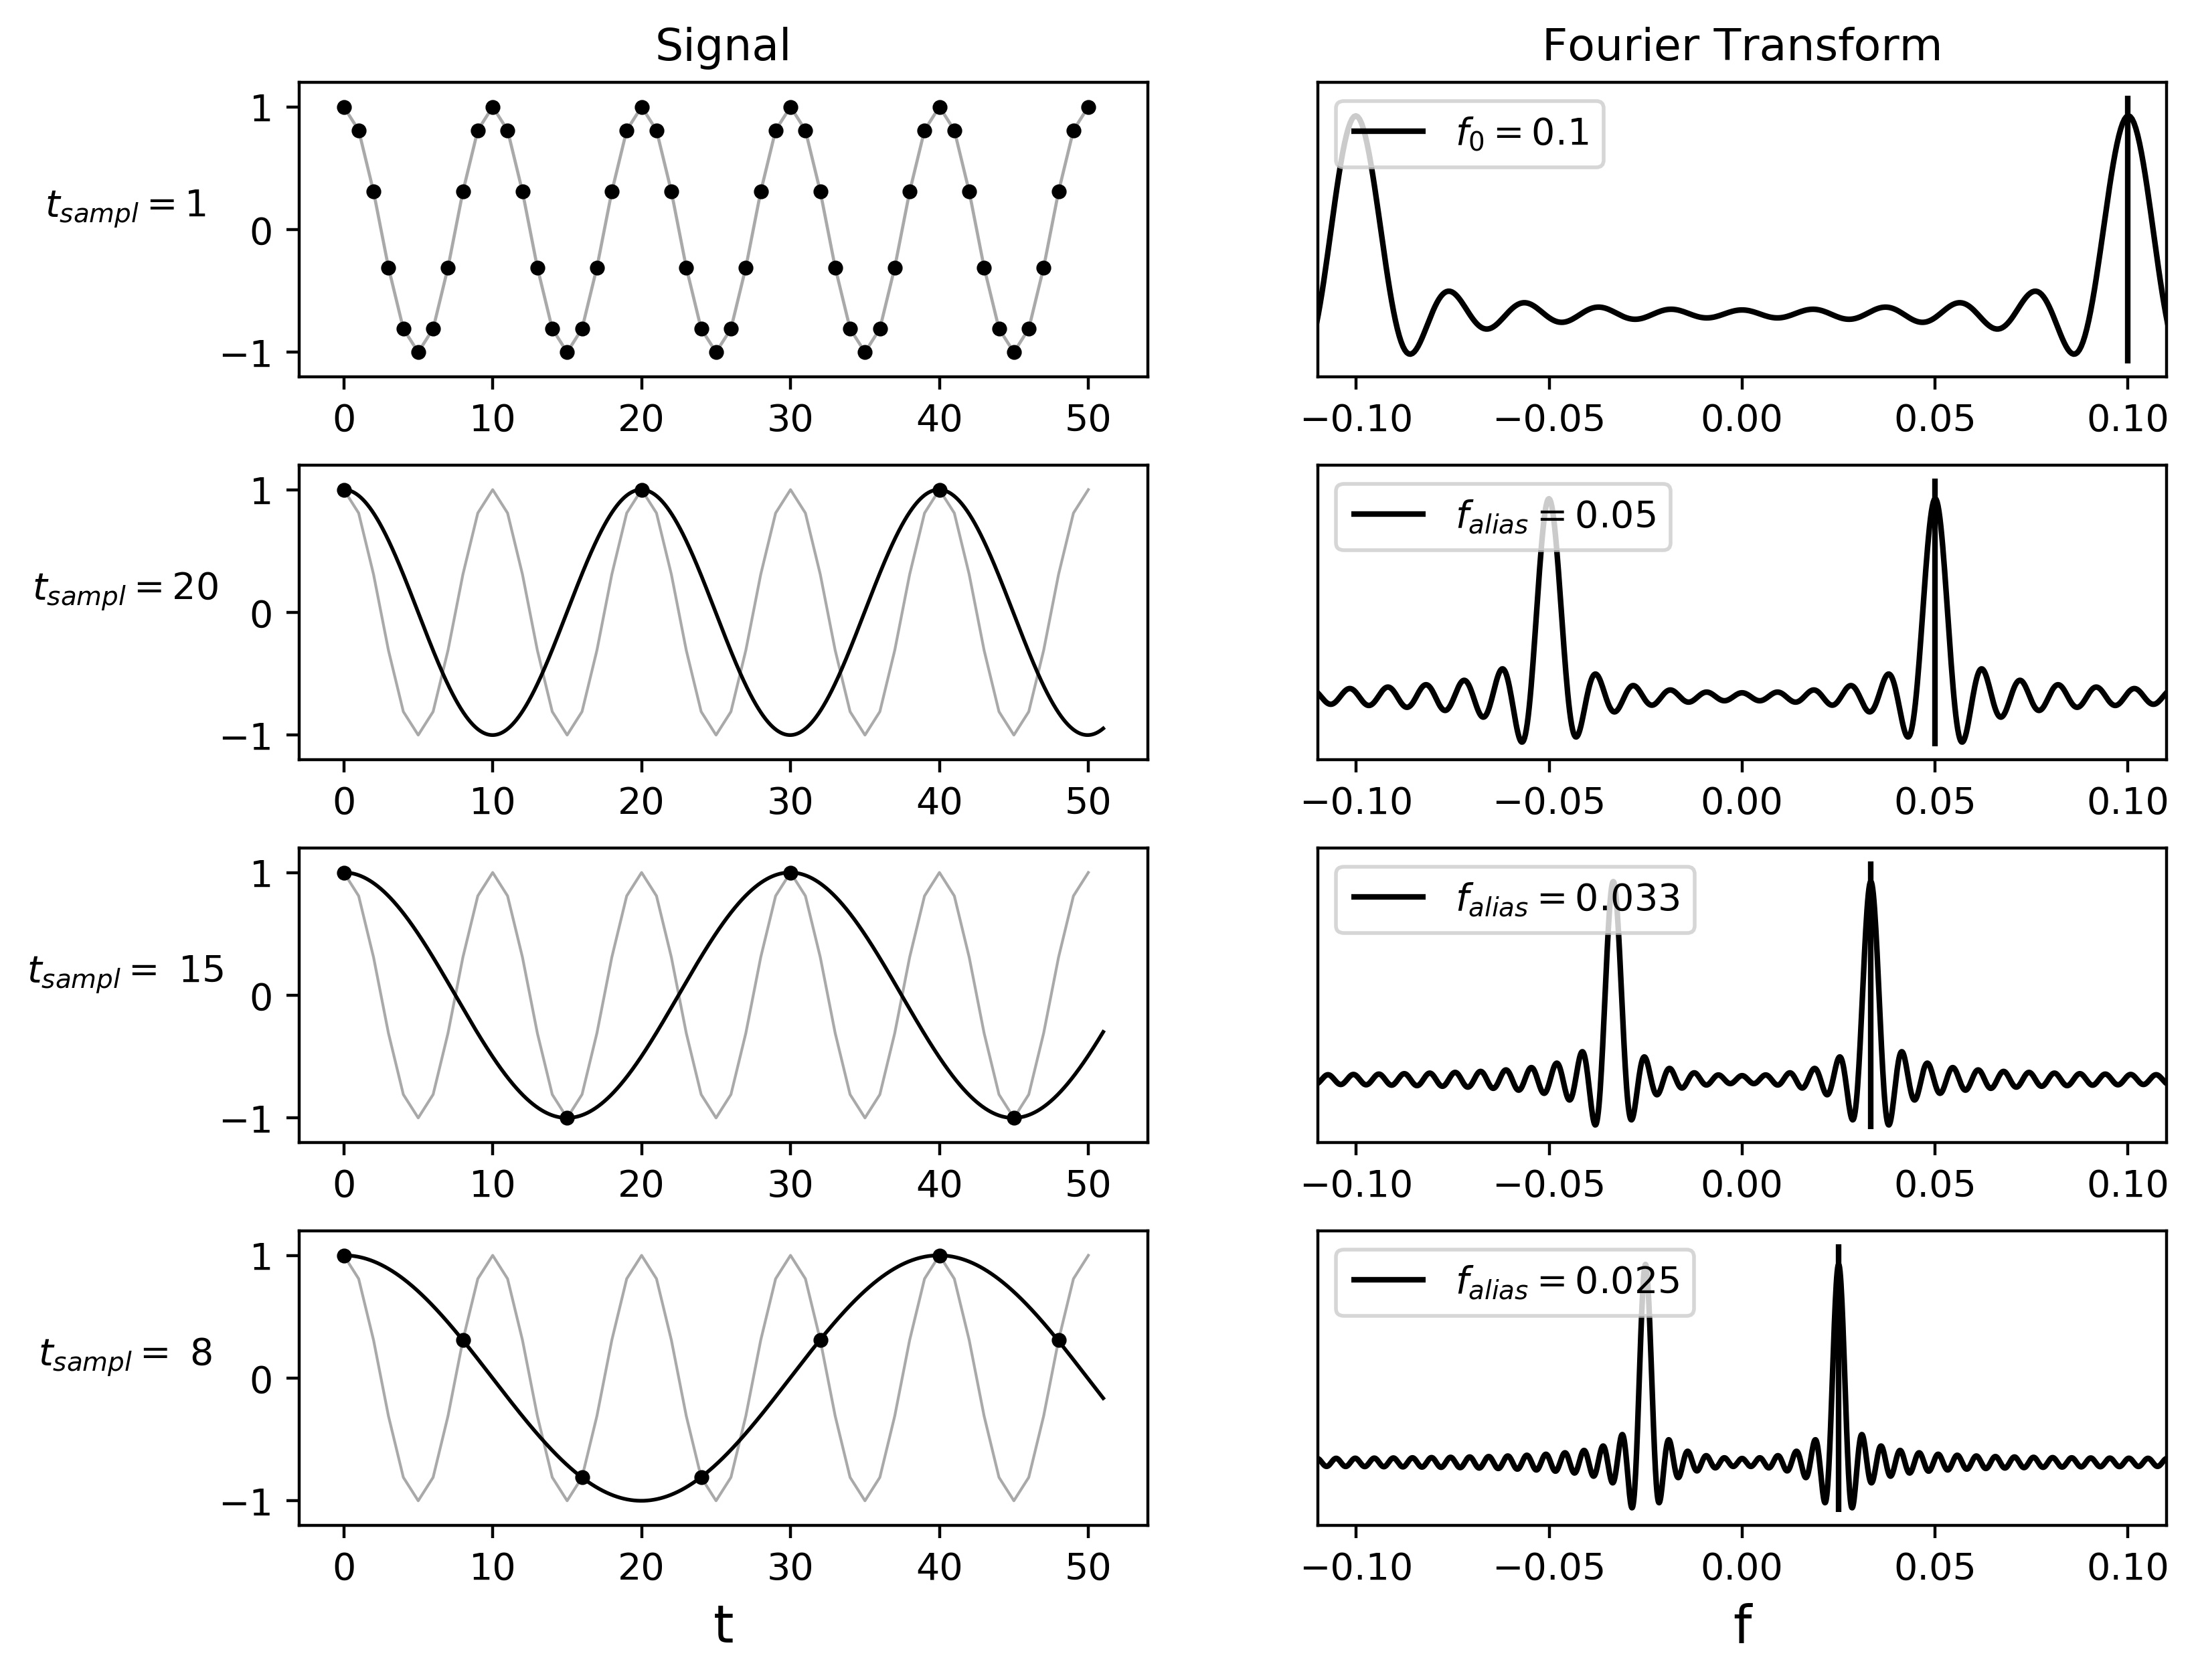
\includegraphics{Figuras/sampling_10.jpg}}
	\end{center}
	\vspace{1mm}	% acrescentar o espaçamento vertical apropriado entre a borda inferior da figura e a legenda ou a fonte quando não há legenda (o valor pode ser negativo para subir)
	\legenda{Efeitos do sampling rate para uma função (ou sinal) cosseno com $f_{0}=0.1$. No topo, o sinal com um sampling rate igual a um. Abaixo, o mesmo sinal sob diferentes sampling rates e suas respectivas transformadas. A linha em cinza claro ilustra o sinal real, e a preta o sinal falsamente identificado tanto pelo nosso cérebro quanto pela FFT, conforme indicado pelos valores de $f_{sampl}$ à direita (todos diferentes de $f_{0}$). Fica evidente que para diferentes taxas, diferentes aliases do sinal original são gerados, de modo que a transformada inversa retornaria um sinal totalmente diferentes do original.} % 	% legenda - para deixar sem legenda usar comando \legenda{} (nunca deve-se comentar o comando \legenda)
	\label{fig:sampling_10}
	%\FONTE{\url{https://omniweb.gsfc.nasa.gov/form/dx1.html}.}	% fonte consultada (elemento obrigatório, mesmo que seja produção do próprio autor)
\end{figure}

\begin{figure}[ht!]
	\caption{Efeitos do sampling rate, $x(t) = \cos(2 \pi /20$, ou seja, $f_{0}=0.05$.}
	\vspace{1mm}	% acrescentar o espaçamento vertical apropriado entre o título e a borda superior da figura
	\begin{center}
		\resizebox{15cm}{!}{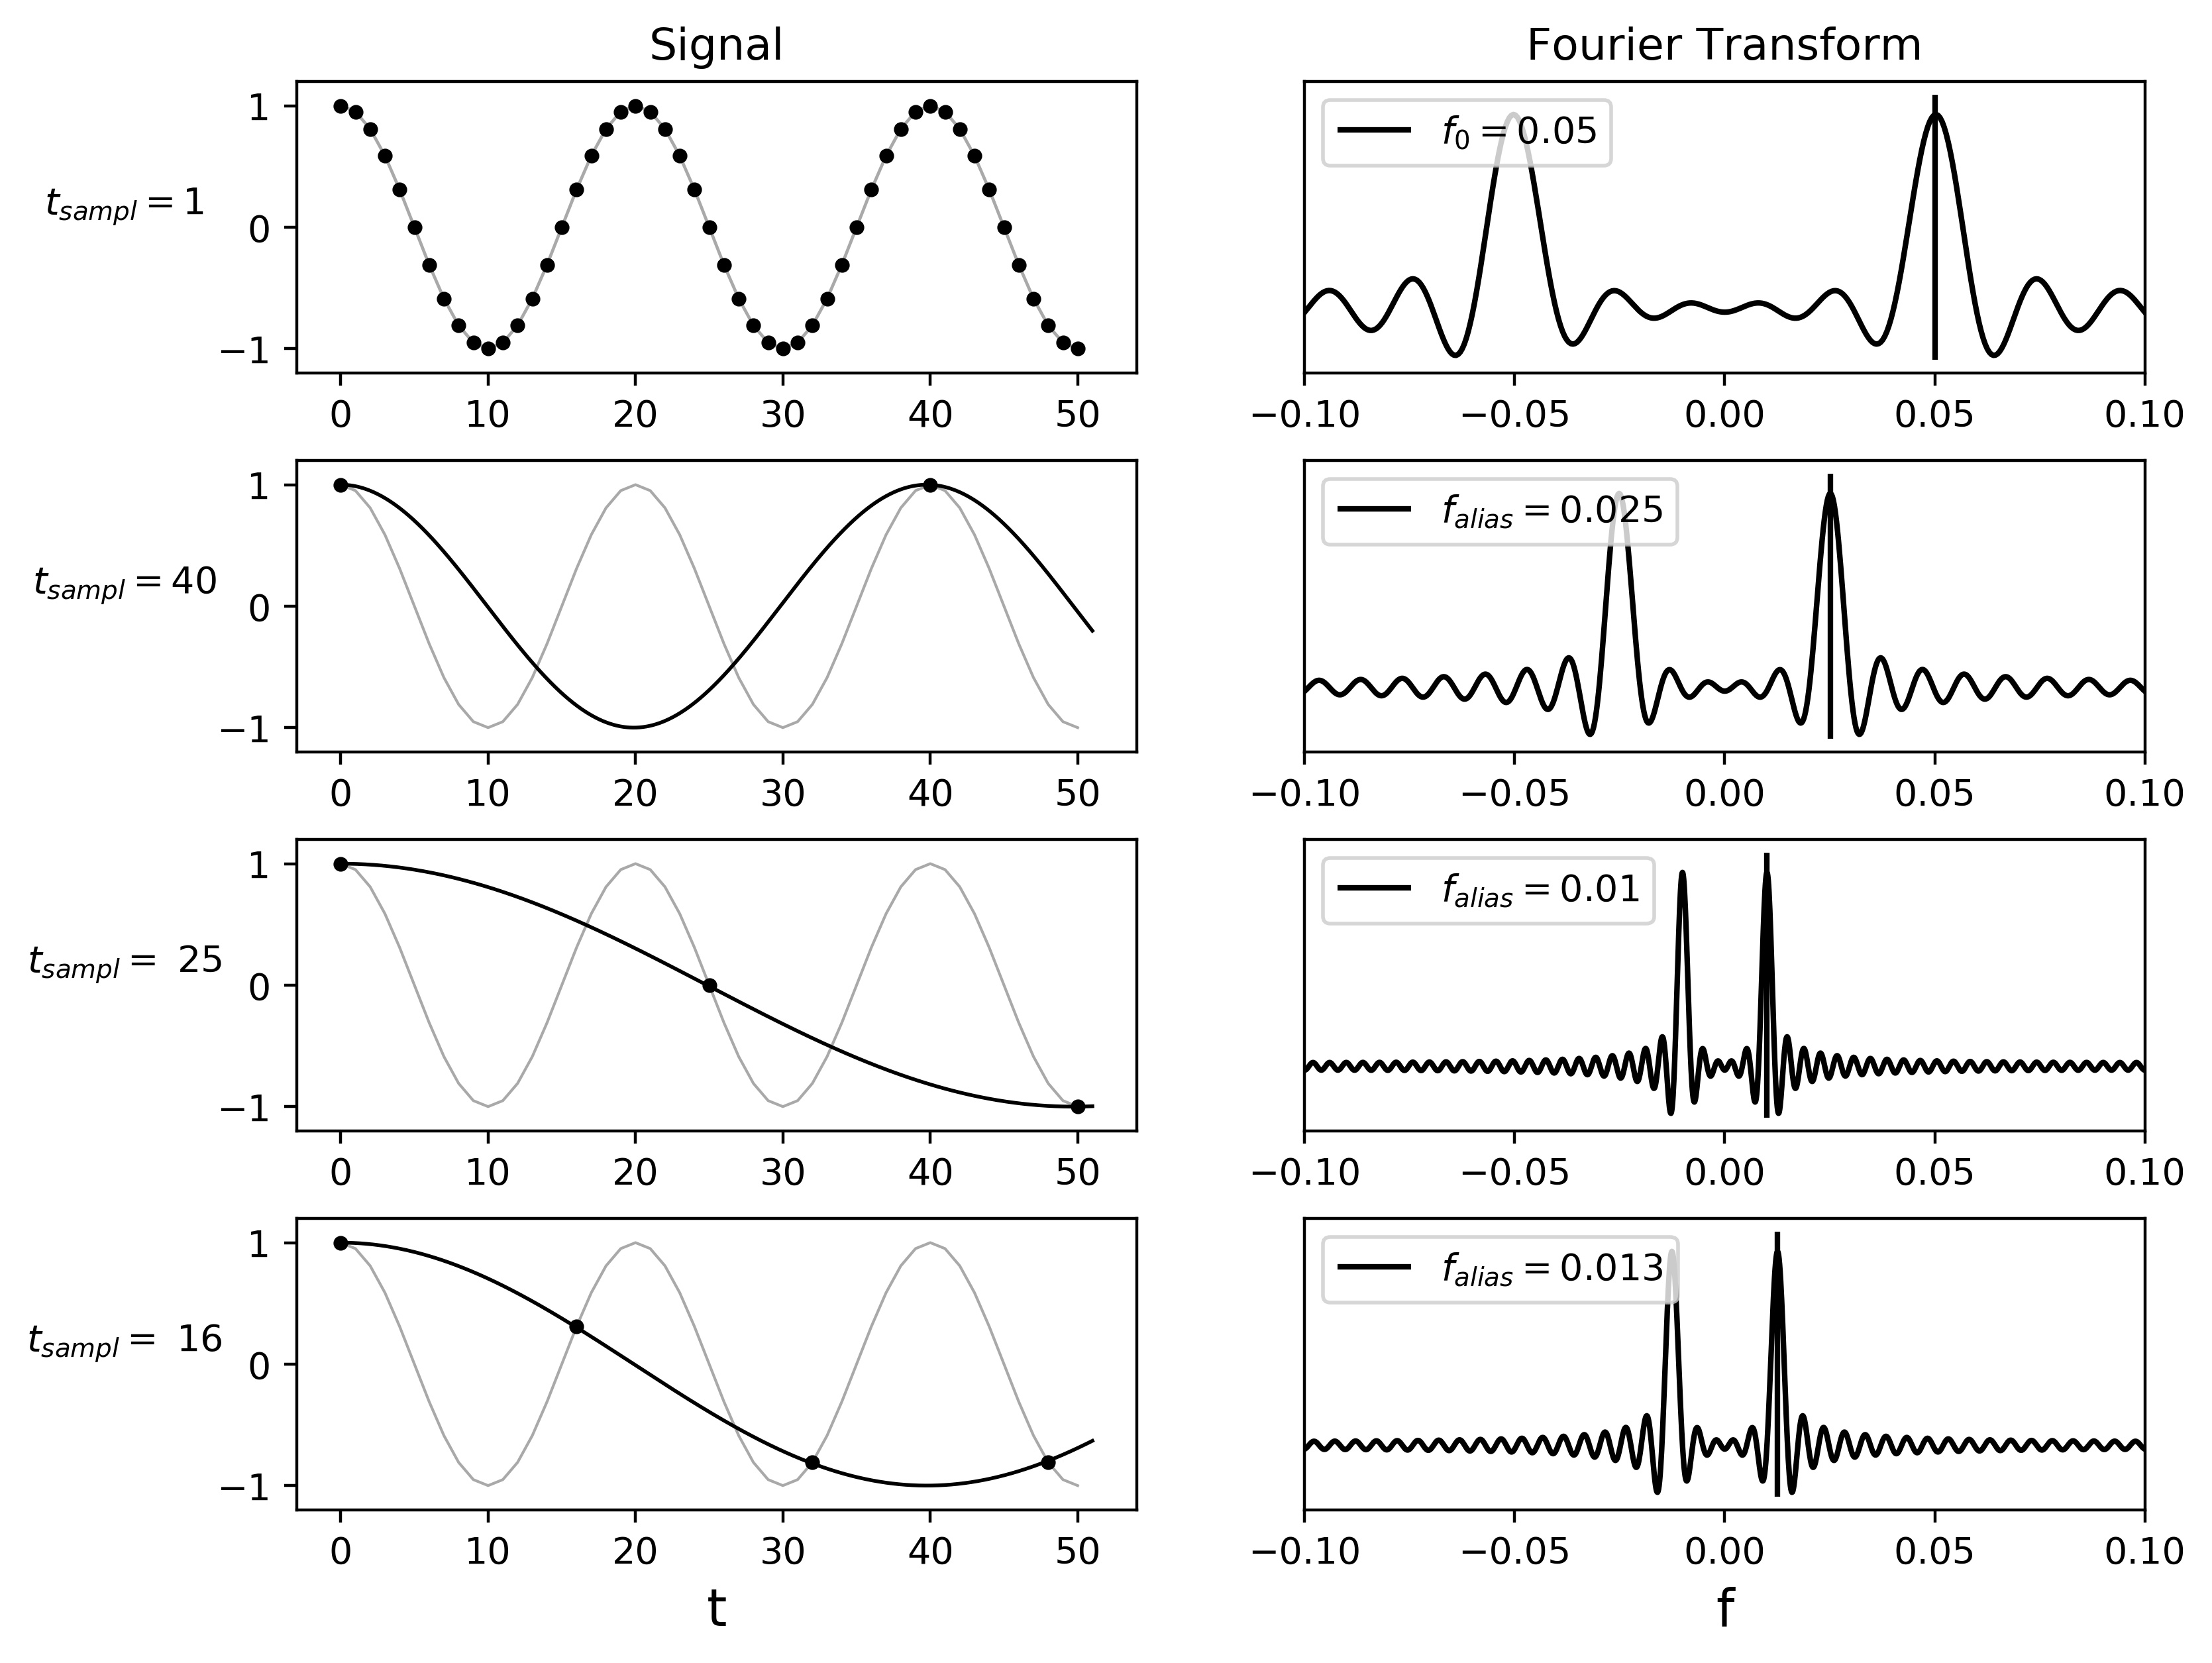
\includegraphics{Figuras/sampling_20.jpg}}
	\end{center}
	\vspace{1mm}	% acrescentar o espaçamento vertical apropriado entre a borda inferior da figura e a legenda ou a fonte quando não há legenda (o valor pode ser negativo para subir)
	\legenda{Efeitos do sampling rate para uma função (ou sinal) cosseno com $f_{0}=0.05$.} % 	% legenda - para deixar sem legenda usar comando \legenda{} (nunca deve-se comentar o comando \legenda)
	\label{fig:sampling_20}
	%\FONTE{\url{https://omniweb.gsfc.nasa.gov/form/dx1.html}.}	% fonte consultada (elemento obrigatório, mesmo que seja produção do próprio autor)
\end{figure}

Porém, se durante uma análise o primeiro passo após receber o sinal fosse produzir sua transformada, observa-se na coluna da direita que a transformada da amostra não condiz com a transformada do sinal original (no topo à direita). A frequência de pico das transformadas não é mais igual a $f_{0}$, de modo que sua transformada inversa resultaria num sinal totalmente diferente do real.

Mais uma vez o efeito da amostragem sobre a transformada pode ser interpretado como a multiplicação do sinal por uma função janela. Aqui a função que multiplica $x(t)$ é uma combinação (somatória) de funções delta espaçadas por $t_{sampl}$, de modo que a Eq. \ref{eq:xobs} se torna:

\begin{equation}
x_{obs}(t) = x(t) \cdot \sum_{n=-\infty}^{\infty}\delta(t - n \cdot t_{sampl}).
\end{equation}

Pelo teorema da convolução:

\begin{equation}
\text{FT}[x_{obs}(t)] = \text{FT}[x(t)] \star \text{FT}[\sum_{n=-\infty}^{\infty}\delta(t - n \cdot t_{sampl})].
\label{eq:conv_app}
\end{equation}

A transformada da combinação de funções delta também é uma combinação de funções delta, desta vez espaçadas por $f_{samp}=1/t_{samp}$ (ver par de transformada da linha de baixo da Figura \ref{fig:adaptado}):

\begin{equation}
\text{FT}[\sum_{n=-\infty}^{\infty}\delta(t - n \cdot t_{sampl})] = \frac{1}{t_{sampl}} \sum_{n=-\infty}^{\infty}\delta(f - n \cdot f_{sampl}),
\end{equation}

e, sendo FT$[x(t)] = X(f)$, a Eq. \ref{eq:conv_app} vira:

\begin{align}
\text{FT}[x_{obs}(t)] &= X(f) \star \left( \frac{1}{t_{sampl}} \sum_{n=-\infty}^{\infty}\delta(f - n \cdot f_{sampl}) \right) \\
 &= \int_{-\infty}^{+\infty} X(s) \frac{1}{t_{sampl}} \sum_{n=-\infty}^{\infty} \delta(f - s - n \cdot f_{sampl}) ds \\
 &= \frac{1}{t_{sampl}}  \sum_{n=-\infty}^{\infty} \int_{-\infty}^{+\infty} X(s) \delta(f - s - n \cdot f_{sampl}) ds \\
 & = \frac{1}{t_{sampl}} \sum_{n=-\infty}^{\infty} X(f - n \cdot f_{sampl}).
\end{align}
%Quanto menor o valor de $t_{samp}$ o efeito é: menor será a capacidade do sinal amostrado exibir características fidedignas do sinal. 

Ou seja, o efeito da frequência de amostragem sobre a transformada de $x(t)$, $X(f)$, é gerar assinaturas falsas em frequências $f_{alias} = |f - N \cdot f_{sampl}|$, onde $N$ é um número inteiro. Por exemplo, nas Figuras \ref{fig:sampling_10} e \ref{fig:sampling_20}, as diferentes frequências falsas são iguais a $f_{alias} = f_{0} - 1/t_{sampl}$. Em particular, na segunda linha da Figura \ref{fig:sampling_10}, para $t_{sampl} = 20$, $f_{alias} = f_{0} - 0.05 = 0.1 - 0.05 = 0.05$, conforme evidenciado pela transformada na coluna da direita. Outro exemplo: na terceira linha da Figura \ref{fig:sampling_20}, tem-se  $t_{sampl} = 25$, e por consequência $f_{alias} = f_{0} - 0.04 = 0.05 - 0.04 = 0.01$. 

Em resumo, a informação sobre $x(t)$ é afetada de modo que sua real forma é perdida, conforme a coluna da esquerda nas Figuras \ref{fig:sampling_10} e \ref{fig:sampling_20} evidencia. A coluna da direita destas Figuras mostra que as diferentes $t_{sampl}$ deram origem a diferentes transformadas de Fourier do mesmo sinal. Outros conceitos relevantes à amostragem e maneiras de evitar aliasing serão discutidos na próxima seção.

%Os lóbulos laterais (leakage spectral) são um artefato devido ao intervalo de observação ser finito. 

\section{Frequência de Nyquist}

Em amostragem discreta, todo sinal possui um limite de largura de banda (\textit{bandwidth}), ou seja, a maior frequência em seu espectro deve estar limitada por um limite superior chamado bandwidth $B$. Portanto, as frequências do sinal estendem-se de 0 a $B$ Hz. Dito isto, é recomendado amostrar o sinal periodicamente à uma taxa alta o suficiente, especificamente $f_{sampl} = 2B$ Hz. Essa ``recomendação'' é conhecida como \textbf{Critério de Nyquist}. Se o critério de Nyquist é violado, o problema de aliasing pode ocorrer. Na seção anterior, para a Figura \ref{fig:sampling_10} (sendo $B = f_{0}$) a frequência de sampling ideal seria $f_{sampl}^{i} = 2 \cdot f_{0} = 2 \cdot 0.1 = 0.2$, correspondendo a um intervalo ideal $t_{sampl}^{i} = 5$. O mais próximo deste valor foi $t_{sampl} = 8$ ou $f_{sampl} = 0.125$ (gráficos de baixo). Já na Figura \ref{fig:sampling_20}, a frequência recomendada seria  $f_{sampl}^{i} = 2 \cdot 0.05 = 0.1$, correspondendo a $t_{sampl}^{i} = 10$, e o mais próximo disto foi $t_{sampl} = 16$ ou $f_{sampl} = 0.0625$ (gráficos de baixo). Em consequência de não se amostrar pelo menos igual mas não acima do $t_{sampl}^{i}$ (ou pelo menos igual mas não abaixo do $f_{sampl}^{i}$) surgem frequências $f_{alias} < f_{0}$.%frequências $f > B$ aparecem em frequências menores. 

Em outras palavras, ao amostrar sob frequência $f_{sampl}$, a frequência máxima que se pode recuperar é igual à metade desta:

\begin{equation}
f_{Ny} = \frac{f_{sampl}}{2},
\end{equation}
que é conhecida como a \textbf{frequência de Nyquist}. Por consequência, a largura de banda do sinal $B$ deve satisfazer $B \leq f_{Ny}$, e esses resultados são conhecidos como \textbf{teorema da amostragem de Nyquist-Shannon}. %Na seção anteior, os sinais das Figuras 3.2 e 3.3 possuíam uma única frequência de modo que esse critério poderia ser facilmente  tinha um frequência única


%\begin{figure}[ht!]
%	\caption{Médias diárias do índice F10.7.}
%	\vspace{0mm}	% acrescentar o espaçamento vertical apropriado entre o título e a borda superior da figura
%	\begin{center}
%		\resizebox{13cm}{!}{\includegraphics{Figuras/jpg_omni2_daily_wSxReptBqw.jpg}}		
%	\end{center}
%	\vspace{-2mm}	% acrescentar o espaçamento vertical apropriado entre a borda inferior da figura e a legenda ou a fonte quando não há legenda (o valor pode ser negativo para subir)
%	\legenda{Médias das medições diárias do fluxo solar. Visualização fornecida pelo portal utilizado para download. Uma análise direta dos dados indicou presença de saltos com valores 999.9, denotando falhas na aquisição. Variações de grande amplitude ocorrem com maior frequência (diariamente), enquanto uma variação global de amplitude média ocorre na escala de alguns anos. O arquivo possui 20440 registros.}	% legenda - para deixar sem legenda usar comando \legenda{} (nunca deve-se comentar o comando \legenda)
%	\label{fig:dailyavg}
%	\FONTE{\url{https://omniweb.gsfc.nasa.gov/form/dx1.html}.}	% fonte consultada (elemento obrigatório, mesmo que seja produção do próprio autor)
%\end{figure}

